\subsection{Shared properties and indiscernibility}
\label{sec:indiscernibility}

\footnote{
  $P$ must be closed under the identity relation, i.e.,
  \begin{equation*}
    cl_{\sim}(P) = \bigcup_{\tuple{\range{p_1}{p_n}} \in P}\nolimits (
      [p_1]_{\sim} \times \ldots \times [p_n]_{\sim}
    )
  \end{equation*}
}

\subsection{Outline of the approach}

We say that two resources are \emph{indiscernible}
  with respect to a set of properties,
  if they share all and only those properties.
We call the properties that a set $X$ of resources shares
  the \emph{indiscernibility criteria} for $X$.
Then we define a new equivalence relation between pairs of resources
  that have the same indiscernibility criteria.
The members of this indiscernibility partition
  have a certain overlap with the original identity relation.
The overlap between an indiscernibility subset and the identity relation
  is called an \emph{identity subrelation}.
For each identity subrelation we can determine the precision,
  defined as the number of identity pairs in the subrelation
  divided by the number of pairs in the subrelation.

\subsubsection{Identity relation -> indiscernibility criteria}

We assume that we are given an identity relation $\approx$,
  which partitions the subject terms according to
  equation \ref{eq:equivalence_set}.

\small
\begin{equation}
\label{eq:equivalence_set}
  \equivset{x}
=
  \setdef{
    y \in S_G
  }{
    \equivpair{x}{y}
  }
\end{equation}
\normalsize

Based on the identity relation, we can derive the properties
  that are shared by a set of resources.
We call the predicates that are shared by a set of identical resources $X$
  the indiscenibility criteria for $X$
  (def. \ref{def:indiscernibility_criteria}).

EXAMPLE HERE (PREFERABLY IIMB).

\begin{definition}[Indiscernibility criteria]
\label{def:indiscernibility_criteria}
\begin{align}
  \indp_{\approx}(\set{\range{x_1}{x_n}})
=
  \setdef{
    p \in P_G
  }{
    \exists_{\range{p_1}{p_n} \in \equivset{p}}(\\
        \equivset{
          \setdef{
            o \in O_G
          }{
            \triple{x_1}{p_1}{o}
          }
        }
      =
        \ldots
      =
        \equivset{
          \setdef{
            o \in O_G
          }{
            \triple{x_n}{p_n}{o}
          }
        }
    )
  }\nonumber
\end{align}
\end{definition}

Notice that in def. \ref{def:indiscernibility_criteria}
  we close both the predicate and object terms under identity.
This results in more shared properties.

\begin{comment}
Drawing:
<s,p,o1>
<s,p,o2>
<o1,=,o2>
From IIMB data.
\end{comment}

\subsection{Identity of typed literals}

In order to assertain that the sets of object terms denote
  the same resources, identity does not suffice due to the special
  conditions for typed literals.
The case here is quite nuanced,
  but typed literals are quite common in SW data,
  so we elaborate on this nuance here.

First we must assume a datatype map
  $D : \mathcal{I} \rightarrow ICEXT(I(\texttt{rdfs:Datatype}))$,
  where $ICEXT$ is the functional mapping from class resources
  to those resources that are instances of that class.
Second, for each datatype $d$ we must assume a lexical-to-value mapping
  $L2V(d) : V(d) \rightarrow LEX(d)$,\cite{Hayes2004}
  and a datatype-specific identity relation on the value space $V(d)$,
  here denoted by $\sim_d$.\footnote{
    Relation $\sim_d$ posed some problems to implement correctly,
    see section \ref{sec:implementation}.}

Suppose that two objects $o_1$ and $o_2$ are both typed literals,
  with $o_1 = \pair{d_1}{x_1}$ and $o_2 = \pair{d_2}{x_2}$
  for datatype names $d_1$ and $d_2$ and value names $x_1$ and $x_2$.
Identity between $o_1$ and $o_2$ is then defined as in
  \ref{def:identity_typed_literals}.

\small
\begin{definition}[Identity for typed literals]
\label{def:identity_typed_literals}
\begin{align}
  o_1 \approx o_1
\,\iff\,
    D(d_1) = D(d_2)
  &\land&\\
    x_1 \in LEX(d_1)
  &\land&\nonumber\\
    x_2 \in LEX(d_2)
  &\land&\nonumber\\
    l2v(D(d_1))(x_1) = l2v(D(d_2))(x_2)\nonumber
\end{align}
\end{definition}
\normalsize

Notice that the datatype-specific lexical-to-value mapping
  in definition \ref{def:identity_typed_literals} is relevant for
  the identification of identity,
  since two lexical expressions may map onto the same value
  according to one datatype but onto different values
  according to another datatype.
An example of this are the lexical expressions $0.1$ and $0.10000000009$,
  which map to the same value according to datatype \texttt{xsd:float}
  but map to different values according to datatype \texttt{xsd:decimal}.

In definition \ref{def:identity_typed_literals} the conjuncts
  stating that the value names belong to the respective lexical spaces
  are not superfluous.
For ill-typed literals,
  i.e. those whose value names do not belong to the lexical space of
  the specified datatype,
  the interpretation is not determined and they are only known to denote
  some arbitrary non-literal value.\footnote{
    From the practice of working with SW data, the authors can testify
    that ill-typed literals do occur and are actually quite common.}

\subsection{Indiscernibility criteria -> identity subrelation}

When we look at the triples that constitute a set of identity relations,
  we see that all identity assertions look the same.
But when we take the properties of those identical resources into account,
  we observe that within a given identity relation there can be different
  subrelations that can be characterized by different sets of properties.

For instance, in the IIMB dataset there are some identical resources that
  share the property \verb|IIMBTBOX:spoken_in|, while other pairs share
  the property \verb|IIMBTBOX:form_of_government|.
The set of pairs of resources that are spoken in the same language may even
  be disjoint from the set of pairs of resources that have the same
  form of government, indicating identity according to different criteria.
In this example, one subset of the identity relation does not discern
  resources that are spoken in the same language, whereas another subset
  of the identity relation does not discern resources that have the same
  form of government.

We say that two resource pairs are indiscernible
  in case both pairs are indiscernible for the same
  $P \subseteq \powerset{P_G}$
  (def. \ref{pair indiscernibility}).

\subsection{Indiscernibility partition -> identity subrelations}

Based on the indiscernibility criteria,
  i.e. the sets of properties that are shared by identical resources,
  we can derive those resource pairs that share
  the same sharing properties.
We can thus identify subsets of an identity relation based on
  differences in the sets of properties relative to which
  the resource pairs that they consist of are
  (in)discernible from one another.
Identity of indiscernibility criteria provides
  another equivalence relation
  ($\approx_{\indp}$, def. \ref{def:indiscernibility_partition}),
  that partitions the identity relation $\approx$ into
  identity subrelations that characterize identity based on different
  indiscernibility criteria.

\begin{definition}[Indiscernibility partition]
\label{def:indiscernibility_partition}
\begin{align}
  \approx_{\indp}
=
  \setdef{
    \pair{\pair{x_1}{x_2}}{\pair{y_1}{y_2}} \in (S_G^2)^2
  }{\\
    \indp_{\approx}(\set{x_1,x_2}) = \indp_{\approx}(\set{y_1,y_2})
  }\nonumber
\end{align}
\end{definition}


\footnote{
  $P$ must be closed under the identity relation, i.e.,
  \begin{equation*}
    cl_{\sim}(P) = \bigcup_{\tuple{\range{p_1}{p_n}} \in P}\nolimits (
      [p_1]_{\sim} \times \ldots \times [p_n]_{\sim}
    )
  \end{equation*}
}

\small
\begin{definition}[Indiscernibility]
\begin{align}
\label{def:resource_indiscernability}
\mathit{IND}(P) \,=\,
  \setdef{
    \pair{x}{y} \in S_G^2
  }{
    \forall_{p \in cl_{\sim}(P)} f_p(x) \approx f_p(y)
  }
\\
\label{pair indiscernibility}
\mathit{IND}(P^*) \,=\,
  \setdef{
    \pair{\pair{x_1}{y_1}}{\pair{x_2}{y_2}} \in (S_G^2)^2
  }{\\
    \forall_{P \in P^*}
        \pair{x_1}{y_1} \in \mathit{IND}(P)
      \leftrightarrow 
        \pair{x_2}{y_2} \in \mathit{IND}(P)
  }\nonumber
\end{align}
\end{definition}
\normalsize

According to the standard definition,
  identical resources are indiscernible with respect to all properties.
We take a given set of identity pairs and partition it into subsets which
  we can describe as being $cl_{\sim}(P)$-indiscernible,
  for $P \subseteq P_G^n$.

Fig. 1 shows an example
  of a discernibility partitioning for a given identity relation.

\begin{comment}
\begin{figure*}
\label{fig:iimb_example}
\centering
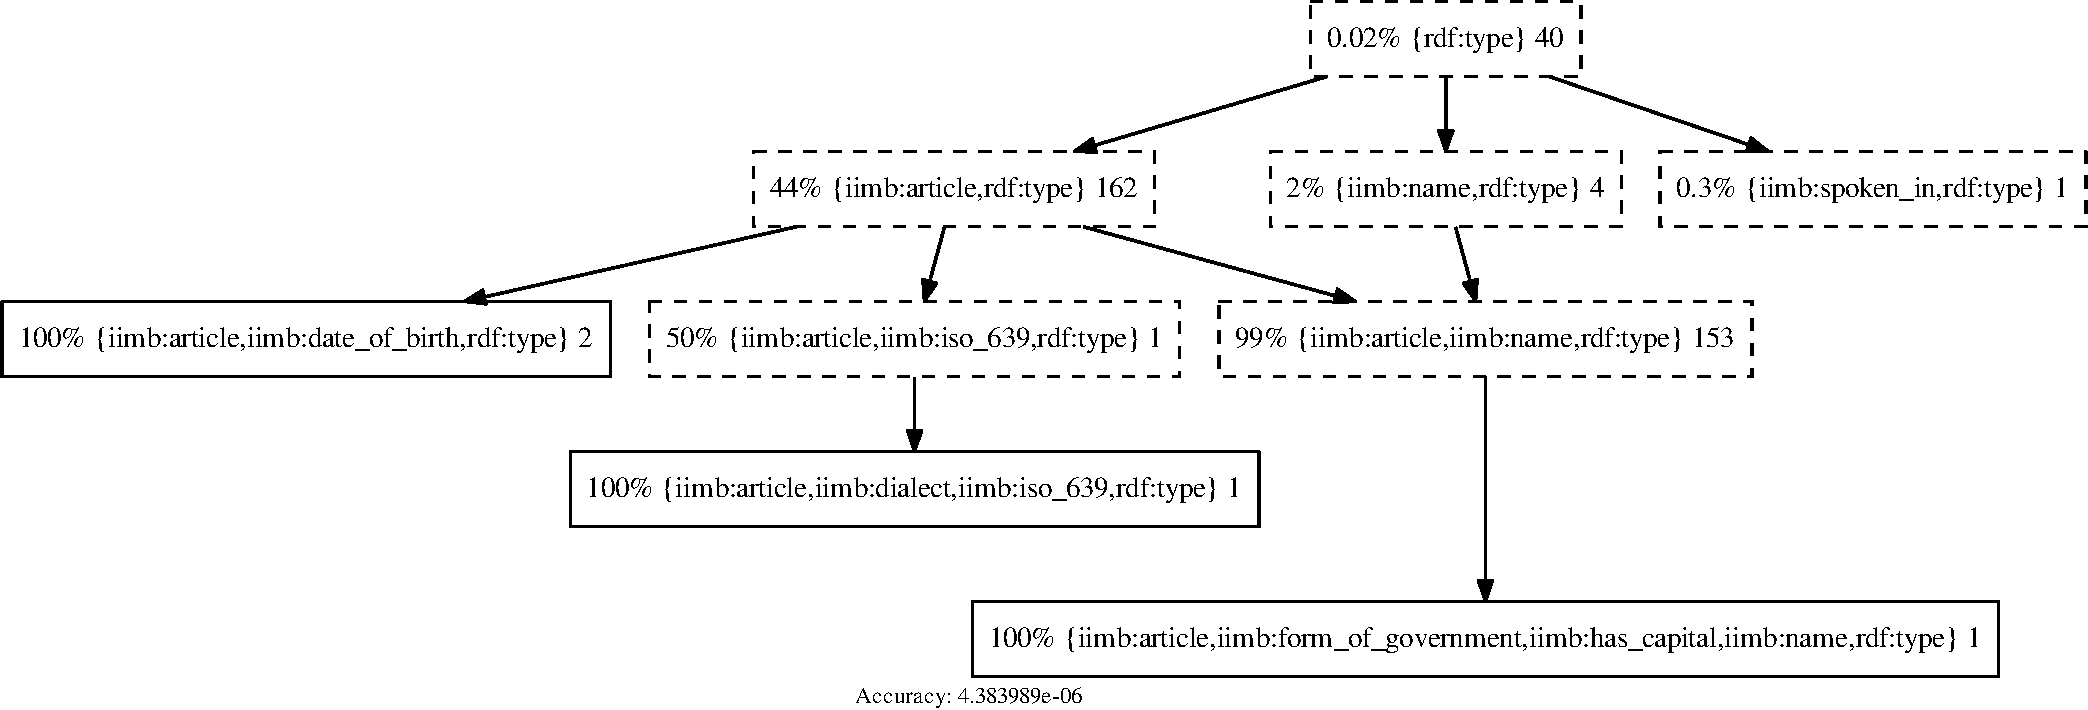
\includegraphics[width=\textwidth]{iimb_approximation_example_crop}
\caption{
  An example of a discernibility partition for an identity relation
    consisting of 365 pairs applied to the fourth IIMB linkset.
  Each node is annotated with the set of predicates $P$ for which
    its pairs are $P$-indiscernible.
  The number of identity pairs within each partition set
    is displayed to the right of the predicate set label.
  Partition sets that contain no identity pair are not show.
  The number that occurs to the left of the predicate label in each node
    indicates how may pairs in that node are identity pairs.
  The lower approximation consists of the nodes with a solid border,
    indicating that they contain only identity pairs.
  The higher approximation consists of all displayed nodes.}
\end{figure*}
\end{comment}
